%! TEX root = ../main.tex
\documentclass[main]{subfiles}

\begin{document}
\chapter{実験方法}
\section{重さの測定}
電子天秤を使って,カーリングブラシパッドの重さを測った.
使用したカーリングブラシパッドの種類は,未使用,10~15投使用,長期間使用の3種類である.
\begin{figure}[htbp]
    \centering
    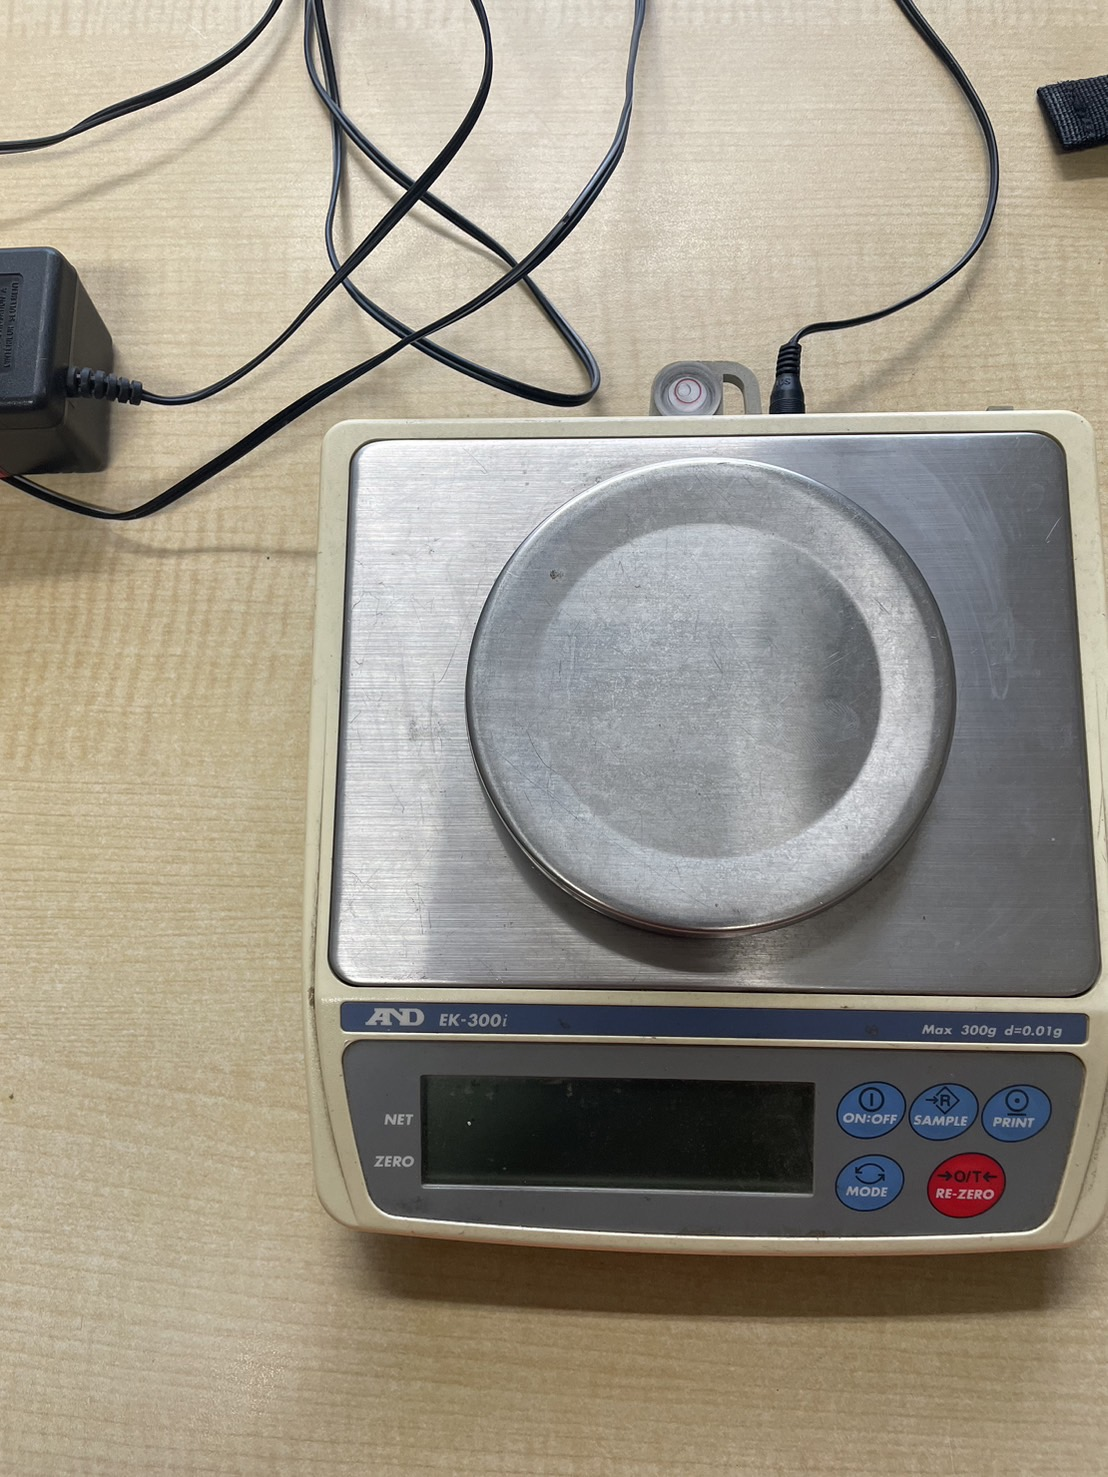
\includegraphics[width=0.5\linewidth, height=0.6\linewidth]{figures/denshitenbinn.jpg}
    \caption{電子天秤}
    \label{fig:label}
\end{figure}

\end{document}